% Options for packages loaded elsewhere
\PassOptionsToPackage{unicode}{hyperref}
\PassOptionsToPackage{hyphens}{url}
%
\documentclass[
  man,floatsintext]{apa7}
\usepackage{amsmath,amssymb}
\usepackage{lmodern}
\usepackage{iftex}
\ifPDFTeX
  \usepackage[T1]{fontenc}
  \usepackage[utf8]{inputenc}
  \usepackage{textcomp} % provide euro and other symbols
\else % if luatex or xetex
  \usepackage{unicode-math}
  \defaultfontfeatures{Scale=MatchLowercase}
  \defaultfontfeatures[\rmfamily]{Ligatures=TeX,Scale=1}
\fi
% Use upquote if available, for straight quotes in verbatim environments
\IfFileExists{upquote.sty}{\usepackage{upquote}}{}
\IfFileExists{microtype.sty}{% use microtype if available
  \usepackage[]{microtype}
  \UseMicrotypeSet[protrusion]{basicmath} % disable protrusion for tt fonts
}{}
\makeatletter
\@ifundefined{KOMAClassName}{% if non-KOMA class
  \IfFileExists{parskip.sty}{%
    \usepackage{parskip}
  }{% else
    \setlength{\parindent}{0pt}
    \setlength{\parskip}{6pt plus 2pt minus 1pt}}
}{% if KOMA class
  \KOMAoptions{parskip=half}}
\makeatother
\usepackage{xcolor}
\IfFileExists{xurl.sty}{\usepackage{xurl}}{} % add URL line breaks if available
\IfFileExists{bookmark.sty}{\usepackage{bookmark}}{\usepackage{hyperref}}
\hypersetup{
  pdftitle={An analysis on Safety and Impact on the Job Market caused by Automation},
  pdfauthor={Rushabh Hitesh Barbhaya1},
  pdflang={en-EN},
  pdfkeywords={Automation, Jobs, Aviation, Self Driving Cars, Engineering, Science, Production, Safety, Lifestyle},
  hidelinks,
  pdfcreator={LaTeX via pandoc}}
\urlstyle{same} % disable monospaced font for URLs
\usepackage{graphicx}
\makeatletter
\def\maxwidth{\ifdim\Gin@nat@width>\linewidth\linewidth\else\Gin@nat@width\fi}
\def\maxheight{\ifdim\Gin@nat@height>\textheight\textheight\else\Gin@nat@height\fi}
\makeatother
% Scale images if necessary, so that they will not overflow the page
% margins by default, and it is still possible to overwrite the defaults
% using explicit options in \includegraphics[width, height, ...]{}
\setkeys{Gin}{width=\maxwidth,height=\maxheight,keepaspectratio}
% Set default figure placement to htbp
\makeatletter
\def\fps@figure{htbp}
\makeatother
\setlength{\emergencystretch}{3em} % prevent overfull lines
\providecommand{\tightlist}{%
  \setlength{\itemsep}{0pt}\setlength{\parskip}{0pt}}
\setcounter{secnumdepth}{-\maxdimen} % remove section numbering
% Make \paragraph and \subparagraph free-standing
\ifx\paragraph\undefined\else
  \let\oldparagraph\paragraph
  \renewcommand{\paragraph}[1]{\oldparagraph{#1}\mbox{}}
\fi
\ifx\subparagraph\undefined\else
  \let\oldsubparagraph\subparagraph
  \renewcommand{\subparagraph}[1]{\oldsubparagraph{#1}\mbox{}}
\fi
\newlength{\cslhangindent}
\setlength{\cslhangindent}{1.5em}
\newlength{\csllabelwidth}
\setlength{\csllabelwidth}{3em}
\newlength{\cslentryspacingunit} % times entry-spacing
\setlength{\cslentryspacingunit}{\parskip}
\newenvironment{CSLReferences}[2] % #1 hanging-ident, #2 entry spacing
 {% don't indent paragraphs
  \setlength{\parindent}{0pt}
  % turn on hanging indent if param 1 is 1
  \ifodd #1
  \let\oldpar\par
  \def\par{\hangindent=\cslhangindent\oldpar}
  \fi
  % set entry spacing
  \setlength{\parskip}{#2\cslentryspacingunit}
 }%
 {}
\usepackage{calc}
\newcommand{\CSLBlock}[1]{#1\hfill\break}
\newcommand{\CSLLeftMargin}[1]{\parbox[t]{\csllabelwidth}{#1}}
\newcommand{\CSLRightInline}[1]{\parbox[t]{\linewidth - \csllabelwidth}{#1}\break}
\newcommand{\CSLIndent}[1]{\hspace{\cslhangindent}#1}
\ifLuaTeX
\usepackage[bidi=basic]{babel}
\else
\usepackage[bidi=default]{babel}
\fi
\babelprovide[main,import]{english}
% get rid of language-specific shorthands (see #6817):
\let\LanguageShortHands\languageshorthands
\def\languageshorthands#1{}
% Manuscript styling
\usepackage{upgreek}
\captionsetup{font=singlespacing,justification=justified}

% Table formatting
\usepackage{longtable}
\usepackage{lscape}
% \usepackage[counterclockwise]{rotating}   % Landscape page setup for large tables
\usepackage{multirow}		% Table styling
\usepackage{tabularx}		% Control Column width
\usepackage[flushleft]{threeparttable}	% Allows for three part tables with a specified notes section
\usepackage{threeparttablex}            % Lets threeparttable work with longtable

% Create new environments so endfloat can handle them
% \newenvironment{ltable}
%   {\begin{landscape}\centering\begin{threeparttable}}
%   {\end{threeparttable}\end{landscape}}
\newenvironment{lltable}{\begin{landscape}\centering\begin{ThreePartTable}}{\end{ThreePartTable}\end{landscape}}

% Enables adjusting longtable caption width to table width
% Solution found at http://golatex.de/longtable-mit-caption-so-breit-wie-die-tabelle-t15767.html
\makeatletter
\newcommand\LastLTentrywidth{1em}
\newlength\longtablewidth
\setlength{\longtablewidth}{1in}
\newcommand{\getlongtablewidth}{\begingroup \ifcsname LT@\roman{LT@tables}\endcsname \global\longtablewidth=0pt \renewcommand{\LT@entry}[2]{\global\advance\longtablewidth by ##2\relax\gdef\LastLTentrywidth{##2}}\@nameuse{LT@\roman{LT@tables}} \fi \endgroup}

% \setlength{\parindent}{0.5in}
% \setlength{\parskip}{0pt plus 0pt minus 0pt}

% Overwrite redefinition of paragraph and subparagraph by the default LaTeX template
% See https://github.com/crsh/papaja/issues/292
\makeatletter
\renewcommand{\paragraph}{\@startsection{paragraph}{4}{\parindent}%
  {0\baselineskip \@plus 0.2ex \@minus 0.2ex}%
  {-1em}%
  {\normalfont\normalsize\bfseries\itshape\typesectitle}}

\renewcommand{\subparagraph}[1]{\@startsection{subparagraph}{5}{1em}%
  {0\baselineskip \@plus 0.2ex \@minus 0.2ex}%
  {-\z@\relax}%
  {\normalfont\normalsize\itshape\hspace{\parindent}{#1}\textit{\addperi}}{\relax}}
\makeatother

% \usepackage{etoolbox}
\makeatletter
\patchcmd{\HyOrg@maketitle}
  {\section{\normalfont\normalsize\abstractname}}
  {\section*{\normalfont\normalsize\abstractname}}
  {}{\typeout{Failed to patch abstract.}}
\patchcmd{\HyOrg@maketitle}
  {\section{\protect\normalfont{\@title}}}
  {\section*{\protect\normalfont{\@title}}}
  {}{\typeout{Failed to patch title.}}
\makeatother

\usepackage{xpatch}
\makeatletter
\xapptocmd\appendix
  {\xapptocmd\section
    {\addcontentsline{toc}{section}{\appendixname\ifoneappendix\else~\theappendix\fi\\: #1}}
    {}{\InnerPatchFailed}%
  }
{}{\PatchFailed}
\keywords{Automation, Jobs, Aviation, Self Driving Cars, Engineering, Science, Production, Safety, Lifestyle\newline\indent Word count: 9}
\usepackage{lineno}

\linenumbers
\usepackage{csquotes}
\usepackage[titles]{tocloft}
\cftpagenumbersoff{figure}
\renewcommand{\cftfigpresnum}{\itshape\figurename\enspace}
\renewcommand{\cftfigaftersnum}{.\space}
\setlength{\cftfigindent}{0pt}
\setlength{\cftafterloftitleskip}{0pt}
\settowidth{\cftfignumwidth}{Figure 10.\qquad}
\cftpagenumbersoff{table}
\renewcommand{\cfttabpresnum}{\itshape\tablename\enspace}
\renewcommand{\cfttabaftersnum}{.\space}
\setlength{\cfttabindent}{0pt}
\setlength{\cftafterloftitleskip}{0pt}
\settowidth{\cfttabnumwidth}{Table 10.\qquad}
\makeatletter
\renewcommand{\paragraph}{\@startsection{paragraph}{4}{\parindent}%
  {0\baselineskip \@plus 0.2ex \@minus 0.2ex}%
  {-1em}%
  {\normalfont\normalsize\bfseries\typesectitle}}

\renewcommand{\subparagraph}[1]{\@startsection{subparagraph}{5}{1em}%
  {0\baselineskip \@plus 0.2ex \@minus 0.2ex}%
  {-\z@\relax}%
  {\normalfont\normalsize\bfseries\itshape\hspace{\parindent}{#1}\textit{\addperi}}{\relax}}
\makeatother

\ifLuaTeX
  \usepackage{selnolig}  % disable illegal ligatures
\fi

\title{An analysis on Safety and Impact on the Job Market caused by Automation}
\author{Rushabh Hitesh Barbhaya\textsuperscript{1}}
\date{}


\shorttitle{Safety and Jobs in Automated World}

\authornote{

This paper is for the Harrisburg University of Science and Technology's graduate course of Analytics GRAD 695 \& ANLY 699. This paper uses actual research for analysis. All the research done by this paper can is reproducible. This document not peer reviewed and peer tested and is therefore for internal use of Harrisburg University of Science and Technology. This research should not be used as a reference in professional study and research.

Correspondence concerning this article should be addressed to Rushabh Hitesh Barbhaya, 326 Market St, Harrisburg, PA 17101. E-mail: \href{mailto:RBarbhaya@my.harrisburgu.edu}{\nolinkurl{RBarbhaya@my.harrisburgu.edu}}

}

\affiliation{\vspace{0.5cm}\textsuperscript{1} Harrisburg University of Science and Technology}

\abstract{%
PlaceHolder
}



\begin{document}
\maketitle

Artificial Intelligence, Machine Learning, Robots, Automation usually outline the news as the cause for mass layoffs, for example, as observed by Mackie (2021). McClure (2018) has similarly observed a correlation between the rise of mainstay automated solutions and growing health and safety concerns. The concern for technology replacing jobs has been known and documented since the 16th century. Hills (1989) and Fleming (2020) notes observe that, in 1589, William Lee's invention of the machine that made stockings had caused a riot in the country. The book ``The Luddites; Machine-Breaking in Regency England,'' authored by Thomis (1972) published in 1972, notes the rise of Luddism. Luddism is a working-class movement asking technology to work with employees and not against them. A modern scripture, ``The Digital Divide'' by Nie and Erbring (2001), has a unique perspective on this. The digital divide refers to the rift caused by a lack of access to information across gender, race, and age, among other demographic keys. Nie and Erbring (2001) observe that the gap is narrowing in current times. Robinson et al. (2003) pushes findings by Nie and Erbring (2001) a bit further and notices the information's bias. However, they do not account for future and future technology.

An article by Smith (2019) states that 50\% of Americans believe that Robots will replace innumerable jobs across the industry. The critical point is that 80\% believe that their jobs will be secure. It seems counterintuitive, but humans always find a more specialized role, which is not surprising. Acemoglu and Autor (2011) outlines the same observations. They observed a decline in low-skilled jobs, raising differences between each level of workers. Acemoglu and Autor (2011) observe that computers replace jobs where cognitive skills and manual input are obligatory. The author did not break down the observations across different industrial sectors where the writer will be observing the results. Authors also published another article Autor et al. (2003), noting an increased skill level of an employee in computer-intense industries. This time the author only focused on technology-focused industries and missed out on observing the same trend across other industrial sectors, which is the focus of this research. Humans also fear ``being left behind,'' says Song (2003), and will always try to cover the skills they offset. Illustrated by other papers in this article, we observe a decline in low-skill jobs that are labor-intensive jobs.

\hypertarget{automation-in-varioius-industires}{%
\section{Automation in varioius industires}\label{automation-in-varioius-industires}}

Abernathy and Townsend (1975) observes the evolution of manual processes. A process that starts as simple logic; evolves into a complex one over time. This complex process generates inefficiencies, and machines are employed to bring back the lost inefficiencies. The author did not account for how these trends are observed in different industrial sectors. Evangelista and Vezzani (2012) balances out the corporate perspective and speaks for human evolution. As robots take on menial jobs, humans find a more specialized roles. Those specialized roles spikes growth and knowledge. Similarly, Bainbridge (1982) describes how automation can work in tandem with humans. Humans can take more managerial roles and let machines handle the rule-based task.

\hypertarget{aviation}{%
\subsection{Aviation}\label{aviation}}

At the time of writing, the airline industry is almost automated. Auto-pilot, take-off and landing assistance, navigation, and other critical functions are automated. However, we still see pilots in the cockpit, monitoring the systems and ensuring everything runs smoothly. Stanton and Marsden (1996) Berberian et al. (2012) also talks about automation in aviation and demonstrates that automation decreases response time and risks. Unfortunately, the authors do not dive much into the increasing reliance on technology, converting the human to a checker role, checking what the robot does, and correcting it for any issues.

\hypertarget{transportation}{%
\subsection{Transportation}\label{transportation}}

The transportation industry is moving towards automated driving systems. (Rice (2019)) Waymo and Tesla are leading that, among others. They are already saving lives, and Lala et al. (2020) shows that the better the automated systems get, the fewer losses to human lives. Schwall et al. (2020), their report mentions the automated systems have already made ways in saving lives. These papers do not talk about what happens if there is an automated car causes an accident. Until driverless cars or self-driving vehicles become a mainstay, Ward (2000) proposes developing an Adaptive Cruise Control system that helps reduce errors and accidents. A need for this cruise control arises because humans have an inherent tendency to make errors as they work on multiple tasks at a time. Having a dedicated machine would help in preventing the loss of lives. The paper does not talk about a merger of these technologies.

\hypertarget{manufacturing}{%
\subsection{Manufacturing}\label{manufacturing}}

The manufacturing industry has utilized robots and artificial intelligence most all the industries. Jämsä-Jounela (2007) talks about how modern industries utilize automation to deliver a reliable product. They use machines anywhere from research and development to marketing the product. The chemical industry is the biggest one. However, the authors missed extending those mechanical knowledge/skills to other industrial sectors.

\hypertarget{healthcare}{%
\subsection{Healthcare}\label{healthcare}}

Automation is also taking its place in healthcare with Machine Learning (ML) and Artificial Intelligence (AI), outlined by Davenport and Kalakota (2019). This article points out the advances ML, and AI have brought to the field. It also points out how a bit of value changes and misdiagnose. ML and AI are still evolving in this field, and the author(s) believe they will have a significant role as the models and data evolve. This paper is an overall approach to future possibilities, current use, current limitations, and live results.

\hypertarget{agriculture}{%
\subsection{Agriculture}\label{agriculture}}

Mahmud et al. (2020) enlighten us about how automation is used in agriculture. Agriculture, at a point in history, was the only job. However, it now has a tiny population engaged in it. Agriculture is probably where automation is heavily relied upon for a consistent output. Additionally, Sarangi et al. (2016) demonstrates how automation is used to deal with crop diseases. Mohanraj et al. (2016) talks about how Internet-of-things can be used to yield a better crop with minimum wastage. A farmer would not be able to monitor their farms without additional help. Internet Of Things could help in those cases and notify any minor change in the field. Also, take measures to avoid harm to the crops. These articles are a good source for understanding how robots and humans can work towards achieving a consistent output and saving time.

\hypertarget{future}{%
\subsection{Future}\label{future}}

We are at such a place in the world where we can deploy another robot to check and validate the other one. Peleska and Siegel (1996) talks about setting a safety standing for reactive systems. Reactive systems kick in when they see an error and try to correct them. The authors proposed a system, when realized, acts as a check before kicking the reactive system of an automation response of a machine. Although, the authors missed the point of humans checking the robot's checked work. Ensure that there are no false positives and false negatives in the response. Daily et al. (2017) looks at how when a machine is released in the real world would be affected by three things. 1. Government regulation, 2. Interference of historical perception to new technologies implementation, and 3. Future. The author missed adding public acceptance of technology. There are many unknowns, but in the end, humans always accept machines as they are convenient and safe. Badue et al. (2021) tests out how each self-driving car's system operates and functions. All the functions they tested were industry standards. Most of the functions of each machine were hidden from the authors, but safety standards were always maintained as per their independent testing.\\

Badue et al. (2021) suggests a hypothetical scenario for self-driving cars and a potential lawsuit. The authors leave an open-ended question after walking through each of the scenarios. The end goal of this exercise is to answer the question, which is to blame when technology is involved in an accident with humans. Strawn (2016) describes an open-ended question about what happens when the future is entirely automated. Will it cause a utopia or a dystopia? Proving sound arguments on both ends.\\

\hypertarget{hypothesis}{%
\subsection{Hypothesis}\label{hypothesis}}

The hypothesis is formulated to extract data from the aviation industry, which is already at a higher level of automation, and translate those results to the motor vehicle industry.

\hypertarget{hypothesis-1}{%
\subsubsection{Hypothesis 1}\label{hypothesis-1}}

Automated systems in the aviation industry result in the loss of jobs.

\hypertarget{hypothesis-2}{%
\subsubsection{Hypothesis 2}\label{hypothesis-2}}

Automated systems in the aviation industry will result in the loss of lives.

\begin{verbatim}
## [1] "### Primary hypothesis\nProcess automation in the finance industry will result in job losses\nThe primary hypothesis will be an extrapolated result from the other hypothesis.\n\n### Hypothesis 1\nAutomated Landing and Piloting systems in the aviation industry results in job loss.\n\n### Hypothesis 2\nAutomated Landing and Piloting systems will raise human safety concerns.\n\n### Hypothesis 3\nSelf-driving and Driverless cars will raise human safety concerns."
\end{verbatim}

\hypertarget{method}{%
\section{Method}\label{method}}

This analysis of extracting data from the aviation industry involves extracting data from various centrally maintained sources. The Department of Transportation, The Bureau of Labor Statistics, and the Department of Transportation Statistics will be used for this analysis.\\

\begin{verbatim}
## [1] "Using the data provided by the United States Bureau Of Labor Statistics (@usbureauoflaborstatistics). The data is sliced by year and industrial section. US Bureau of Labor Statistics houses data in multiple formats, using simple flat files for this analysis. US Bureau of Labor Statistics also provides with data key to decode the column names. Similarly, safety data is also obtained from government agencies. IATA @iata provides a safety report across years for this analysis. Department of Transportation provides road safety reports. Data will be combined from official government-managed websites and other sources that confirm when automation was implemented in that industry. For example, Auto-Pilot was invented in 1912 @windsor1913popular with its initial implementation in 1970 following the Lunar Landing Module @widnall1971lunar. \nFollowing the results from these sections, the results are trend analyzed and extrapolated to the finance industry to conclude the suggested hypothesis. *\n\n## Participants\nAbsolute numbers from the statistics reports as the participants in this analysis. These reports are ranged from 1930 to 2020. The key column in this report being the unemployment rate across industries and safety reports. \nThe reports and articles from multiple sources will be utilized to check if a robotic process resulted in a loss of jobs and loss of lives. Or was it the loss of lives and loss of jobs that gave rise to robots?"
\end{verbatim}

\hypertarget{procedures}{%
\subsection{Procedures}\label{procedures}}

The first step in this analysis is to clean, treat outliers and normalize the data. Cleaning the data entails checking for formatting issues, excluding unwanted data that impact execution speed. A correctly formatting the data to the correct data type used in the analysis. Converting percent to 0-1 normalized values wherever required to improve the speed of the analysis.\\

Outliers are subjective. Outliers affect the final results of the analysis. Outliers may skew the results in any direction; therefore, it becomes essential to identify and treat them accordingly.\\
It is essential to normalize data that spans multiple years to a joint base. Treating safety reports and employment records to parts per thousand is the first step before performing any analysis. This makes a comparison on equal terms.\\

\begin{verbatim}
## [1] "## Measures\nFor the hypothesis tests, the confidence interval is set at 90% as there are for almost a century which may result in a more significant change. The measure of success is calculated on p-values from the hypothesis testing with an acceptable p-value of less than or equal to 0.01 and significant variables from the analysis. \nThese results are weighted and applied to the finance industry, which is the basis for this research. The weighing factor is ranged from 0 to 1 and is fed to a Monte Carlo series to account for any random error which may occur. \n\n## Analysis\nThe overall mean from the Monte Carlo simulation results is compared with the trends in technology, aviation, manufacturing, and agriculture industries. This result will not only give the current position on the automation trend but also give an estimate. Estimation of how long it would take for robots to be accepted in this industry. Monte Carlo series helps normalize and accounts for any random error that may occur. \nR (@R-base) is used to extract all the results, except the Monte Carlo simulation. Monte Carlo simulation is performed by python (@python.org_2021)."
\end{verbatim}

\hypertarget{tools-of-automation}{%
\subsection{Tools of automation}\label{tools-of-automation}}

{``The r Project for Statistical Computing''} (2022) with Aust and Barth (2022) are used to create this paper and {``Python Release Python 3.9.7''} (2021) for modeling and plotting graphs for these analyses.\\

\hypertarget{aviation-industry}{%
\subsection{Aviation Industry}\label{aviation-industry}}

The focus of this paper is to extract and generate insights from the heavily automated aviation industry and speculate on the results of the motor vehicle industry. The motor vehicle industry is steadily moving towards complete automation. Beresnevicius (2019) analysis says that the flying, landing, breaking, and take off are already automated in the commercial aviation industry. When writing this paper, Tesla and Waymo are already testing out their version of ``auto-pilot'' systems. These ``auto-pilot'' or self-driving features move the driver from an active role to a passive role. US Department of Transportation and National Highway Traffic Safety Administration Administration (n.d.) have documented a roadmap for moving to utterly automated driving. They have categorized levels of automated driving from Level 0 to Level 5.\\

Level 0 is ``Momentary Driver Assistance,'' things like warning lights and notifications. Level 1 is ``Driver Assistance''; the vehicle provides some assistance to the driver. Adaptive cruise control and lane assistance are some examples of Level 1 assistance. Level 2 is ``Additional Assistance'' here, and the vehicle assists in acceleration, braking, also steering. Level 3 is ``Conditional Automation'' we have not reached this level of automation at the time of this article. Level 3 is where the system takes over, and a driver must be behind the wheel to take over at any point. Waymo and Tesla are piloting this system but are not entirely out of testing yet. Level 4 is ``High automation'' this level of automation is where there is no need for a human driver under some conditions. Humans can act as passengers in this level of automation. Level 5 is ``Full Automation''; here, there is no need for a human driver. Systems are wholly automated at all levels and conditions. The automation levels mentioned put the aviation industry at level 4 automation. The pilots are mostly monitoring systems that are in place to help the airline fly safely but take over whenever needed.\\

The aviation data is divided into three segments; 1. The number of flights that have taken off in the USA, 2. Aviation incidents through history, and 3. History of jobs in the aviation industry.\\

\hypertarget{flights-in-the-usa}{%
\subsubsection{Flights in the USA}\label{flights-in-the-usa}}

For understanding the automation industry, it is important to understand the number of flights that have taken off from the land of the USA. It, directly and indirectly, gives us a sense of how the population perceives the aviation industry as a whole. One of the factors for understanding safety in the aviation industry would be utilizing the services. Economics and logistics are also important factors in the industry, but they do not fall within the scope of this research. The data for getting the number of flights in the USA was downloaded from Transportation Statistics (2022), and the key for the data was derived from Blevins (2010). The description of the table \ref{tab:aviation-flights}\\

\begin{table}[tbp]

\begin{center}
\begin{threeparttable}

\caption{\label{tab:aviation-flights}Domestic flights from 1990 to 2021 for all the major airlines in the USA}

\begin{tabular}{lll}
\toprule
Column & \multicolumn{1}{c}{Context} & \multicolumn{1}{c}{Datatype}\\
\midrule
Carrier & Unique value of the airline carrier & string\\
Carrier Name & Full name of the airline carrier & string\\
Origin Airport ID & Code of the airport from where the aircraft took flight & interger\\
Origin & Name of the place the airline took off & string\\
Destination Airport ID & Code of the airport where the aircraft landed & interger\\
Destination & Full name of the destination airport & string\\
Year & Timestamp of when the aircraft took flight & date(YYYY)\\
Month & Timestamp of when the aircraft took flight & date(MM)\\
\bottomrule
\addlinespace
\end{tabular}

\begin{tablenotes}[para]
\normalsize{\textit{Note.} This table has 6801406 rows and 9 columns}
\end{tablenotes}

\end{threeparttable}
\end{center}

\end{table}

\begin{figure}

{\centering 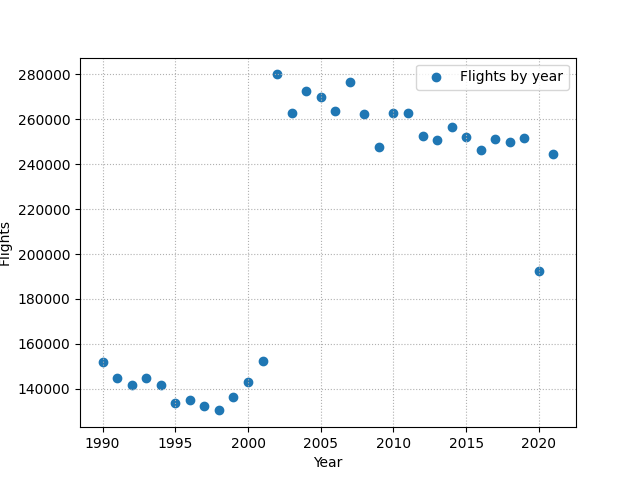
\includegraphics{./graphs/Count of flights} 

}

\caption{Trend of domestic flights in the USA}\label{fig:aviation-flights-image}
\end{figure}

\begin{table}[tbp]

\begin{center}
\begin{threeparttable}

\caption{\label{tab:aviation-jobs-schema}Trend of jobs in the aviation industry}

\begin{tabular}{lll}
\toprule
column & \multicolumn{1}{c}{Context} & \multicolumn{1}{c}{format}\\
\midrule
ID & Unique identifier for each year & string\\
Year & Year for the statictic & date(YYYY)\\
Period & Month of the statictic & string(date(MM))\\
Label & Month and Year combined for label & string\\
Value & Year "1" acts as benchmark and subsequest year shows the & float\\
 & percent increase/decrease in employement numbers & \\
\bottomrule
\end{tabular}

\end{threeparttable}
\end{center}

\end{table}

\begin{table}[tbp]

\begin{center}
\begin{threeparttable}

\caption{\label{tab:aviation-incidents-schema}Trend of incidents in the aviation industry, scope limited to the USA}

\begin{tabular}{lll}
\toprule
column & \multicolumn{1}{c}{description} & \multicolumn{1}{c}{fieldtype}\\
\midrule
Data dimension & Data dimension from source & 168461 x 14\\
Scope limited data & Data dimension after limiting the scope USA & 151665 x 14\\
Duplicates removed & Data after removing duplicates & 80728 x 14\\
event id & Unique identifier for the event & string\\
ntsb number & Unique identifier created by the NTSB & string\\
event state & Name of the state where the event occured & string(2)\\
event country & Country of the state where the event occured & string(3)\\
event year & Year (timestamp) of the event & integer(date:YYYY)\\
event month & Month (timestamp) of the event & integer(date:MM)\\
fatal injuries on ground & Fatalities on ground of the event site & integer\\
minor injuries on ground & Minor injuries at the event site & integer\\
serious injuries on\ \ ground & Serious injuries at the event site & integer\\
total injuries on flight & Total injuries on flight & integer\\
minor injuries in flight & Fatal injuries on flight & integer\\
serious injuries in flight & Minor injuries on flight & integer\\
fatal injures in flight & Serious injuries on flight & integer\\
total ground injuries & Calculated Field: Total ground injuries & integer\\
total flight injuries & Calculated Field: Total flight injuries & integer\\
total injuries & Calculated Field: Total injuries & integer\\
\bottomrule
\end{tabular}

\end{threeparttable}
\end{center}

\end{table}

\begin{figure}

{\centering 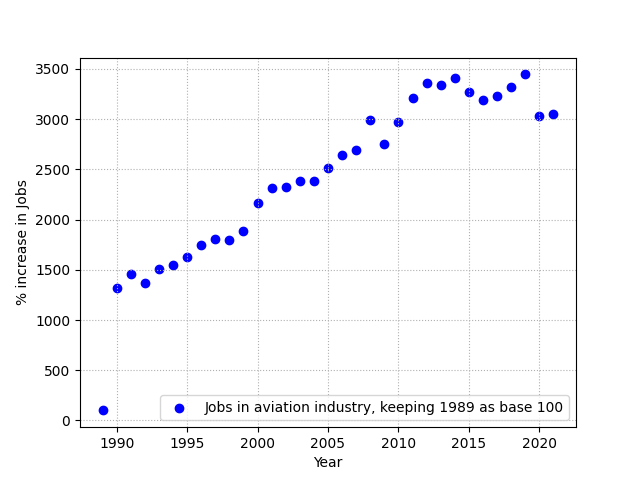
\includegraphics{./graphs/Jobs in the aviation industry} 

}

\caption{Trend of aviation jobs over the years}\label{fig:aviation-jobs-image}
\end{figure}

\begin{figure}

{\centering 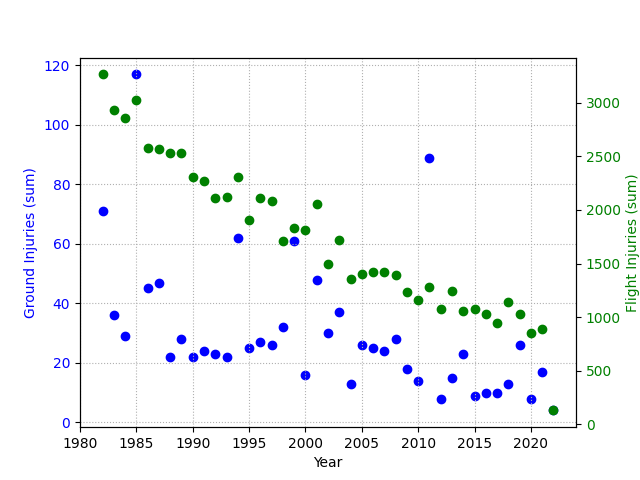
\includegraphics{./graphs/flight_injuries} 

}

\caption{Trend of injuries across time}\label{fig:aviation-incident-plot}
\end{figure}

The table \ref{tab:aviation-flights} is a scoped table used for the analysis. There are no \texttt{NULL} or \texttt{empty} values in the table and therefore do not need to be treated for it. Therefore, this data is derived from official sources and should not be scoped for outliers. To see the trend for the number of flights in the USA, refer to figure \ref{fig:aviation-flights-image}. The figure is grouped by the year, and a count of total flights is demonstrated in the figure \ref{fig:aviation-flights-image}\\
The flights in the domestic USA had a sudden rise around 2002. With a significant dip in the year 2020 on account of the global pandemic of COVID-19. The following year, the number of flights jumped back to its ``normal'' trend.

\hypertarget{jobs-in-the-aviation-industry}{%
\subsubsection{Jobs in the aviation industry}\label{jobs-in-the-aviation-industry}}

To measure how automation has affected the aviation industry, it is to look at the jobs in the aviation industry. The Bureau of Labor Statistics Labor Statistics (2022) provides the data for this analysis. The data schema is shown in the table \ref{tab:aviation-jobs-schema}. There are no \texttt{NULL} or \texttt{empty} values in the data; hence cleanup is not required. This data comes directly from the Bureau of Labor Statistics and is not scoped for outliers.\\

The data is grouped by year and then summed for each year. This will give us the trend for aviation jobs across the USA. From the trend, the number of jobs in the aviation industry seems to be increasing over the years, shown in figure \ref{fig:aviation-jobs-image}\\

\hypertarget{incidents-in-the-aviation-industry}{%
\subsubsection{Incidents in the aviation industry}\label{incidents-in-the-aviation-industry}}

After any incident in any aviation industry, a new safety standard is observed. New automation opportunity arises from these safety standards. Auto-pilot was introduced for long flights to relieve pilots from fatigue. Take-off and landing assistance were introduced to combat climatic factors at the airports. Overall the safety standards increase following incidents. Board (2022) provides us with the incident figures with the count of fatalities and injuries. The overall dataset facts are stated in the table \ref{tab:aviation-incidents-schema}\\

The dataset contains \texttt{NULL} in the integer columns. Those are equated to \texttt{0} for calculated columns. \texttt{Total\ Ground\ Injures} and \texttt{Total\ Flight\ Injuries} are calculated columns to understand the trend of injuries across \texttt{year,} displayed in figure \ref{fig:aviation-incident-plot}\\

The plot shows the downward trend of injuries, both in flight and on the ground. The blue plots show the number of ground injuries over the years, and the green plots show the number of flight injuries. This is a dual-axis graph to indicate the number of injuries from 1981 to 2021\\

\newpage

\hypertarget{references}{%
\section{References}\label{references}}

\begingroup
\setlength{\parindent}{-0.5in}
\setlength{\leftskip}{0.5in}

\hypertarget{refs}{}
\begin{CSLReferences}{1}{0}
\leavevmode\vadjust pre{\hypertarget{ref-abernathy1975technology}{}}%
Abernathy, W. J., \& Townsend, P. L. (1975). Technology, productivity and process change. \emph{Technological Forecasting and Social Change}, \emph{7}(4), 379--396.

\leavevmode\vadjust pre{\hypertarget{ref-acemoglu2011skills}{}}%
Acemoglu, D., \& Autor, D. (2011). Skills, tasks and technologies: Implications for employment and earnings. In \emph{Handbook of labor economics} (Vol. 4, pp. 1043--1171). Elsevier.

\leavevmode\vadjust pre{\hypertarget{ref-levelsofautomation}{}}%
Administration, N. H. T. S. (n.d.). \emph{The evolution of automated safety technologies}. US Department of Transportation. \url{https://www.nhtsa.gov/technology-innovation/automated-vehicles-safety}

\leavevmode\vadjust pre{\hypertarget{ref-R-papaja}{}}%
Aust, F., \& Barth, M. (2022). \emph{{papaja}: {Prepare} reproducible {APA} journal articles with {R Markdown}}. \url{https://github.com/crsh/papaja}

\leavevmode\vadjust pre{\hypertarget{ref-autor2003skill}{}}%
Autor, D. H., Levy, F., \& Murnane, R. J. (2003). The skill content of recent technological change: An empirical exploration. \emph{The Quarterly Journal of Economics}, \emph{118}(4), 1279--1333.

\leavevmode\vadjust pre{\hypertarget{ref-badue2021self}{}}%
Badue, C., Guidolini, R., Carneiro, R. V., Azevedo, P., Cardoso, V. B., Forechi, A., Jesus, L., Berriel, R., Paixao, T. M., Mutz, F.others. (2021). Self-driving cars: A survey. \emph{Expert Systems with Applications}, \emph{165}, 113816.

\leavevmode\vadjust pre{\hypertarget{ref-bainbridge1982ironies}{}}%
Bainbridge, L. (1982). Ironies of automation. \emph{IFAC Proceedings Volumes}, \emph{15}(6), 129--135.

\leavevmode\vadjust pre{\hypertarget{ref-berberian2012automation}{}}%
Berberian, B., Sarrazin, J.-C., Le Blaye, P., \& Haggard, P. (2012). Automation technology and sense of control: A window on human agency. \emph{PloS One}, \emph{7}(3), e34075.

\leavevmode\vadjust pre{\hypertarget{ref-beresnevicius_2019}{}}%
Beresnevicius, R. (2019). Automation in the aviation industry - the future is automated. In \emph{AeroTime Hub}. AeroTime Hub. \url{https://www.aerotime.aero/articles/23162-automation-aviation-industry}

\leavevmode\vadjust pre{\hypertarget{ref-AirlineI37}{}}%
Blevins, J. (2010). \emph{Airline industry datasets}. \url{https://jblevins.org/notes/airline-data}.

\leavevmode\vadjust pre{\hypertarget{ref-Accident29}{}}%
Board, N. T. S. (2022). \emph{Accident data}. \url{https://www.ntsb.gov/safety/data/Pages/Data_Stats.aspx}.

\leavevmode\vadjust pre{\hypertarget{ref-daily2017self}{}}%
Daily, M., Medasani, S., Behringer, R., \& Trivedi, M. (2017). Self-driving cars. \emph{Computer}, \emph{50}(12), 18--23.

\leavevmode\vadjust pre{\hypertarget{ref-davenport2019potential}{}}%
Davenport, T., \& Kalakota, R. (2019). The potential for artificial intelligence in healthcare. \emph{Future Healthcare Journal}, \emph{6}(2), 94.

\leavevmode\vadjust pre{\hypertarget{ref-evangelista2012impact}{}}%
Evangelista, R., \& Vezzani, A. (2012). The impact of technological and organizational innovations on employment in european firms. \emph{Industrial and Corporate Change}, \emph{21}(4), 871--899.

\leavevmode\vadjust pre{\hypertarget{ref-fleming2020short}{}}%
Fleming, S. (2020). \emph{A short history of jobs and automation}.

\leavevmode\vadjust pre{\hypertarget{ref-hills1989william}{}}%
Hills, R. L. (1989). William lee and his knitting machine. \emph{Journal of the Textile Institute}, \emph{80}(2), 169--184.

\leavevmode\vadjust pre{\hypertarget{ref-jamsa2007future}{}}%
Jämsä-Jounela, S.-L. (2007). Future trends in process automation. \emph{Annual Reviews in Control}, \emph{31}(2), 211--220.

\leavevmode\vadjust pre{\hypertarget{ref-BLSDataV82}{}}%
Labor Statistics, U. S. B. of. (2022). \emph{BLS data viewer}. \url{https://beta.bls.gov/dataViewer/view/timeseries/PCU481---481---}.

\leavevmode\vadjust pre{\hypertarget{ref-lala2020autonomous}{}}%
Lala, J. H., Landwehr, C. E., \& Meyer, J. F. (2020). Autonomous vehicle safety: Lessons from aviation. \emph{Communications of the ACM}, \emph{63}(9), 28--31.

\leavevmode\vadjust pre{\hypertarget{ref-mackie_2021}{}}%
Mackie, C. (2021). Beware professional services workers: Robots are coming for your job too! In \emph{Forbes}. Forbes Magazine. \url{https://www.forbes.com/sites/calvinmackie/2021/09/30/beware-professional-services-workers-robots-are-coming-for-your-job-too/?sh=2fd2aa5b5237}

\leavevmode\vadjust pre{\hypertarget{ref-mahmud2020robotics}{}}%
Mahmud, M. S. A., Abidin, M. S. Z., Emmanuel, A. A., \& Hasan, H. S. (2020). Robotics and automation in agriculture: Present and future applications. \emph{Applications of Modelling and Simulation}, \emph{4}, 130--140.

\leavevmode\vadjust pre{\hypertarget{ref-mcclure2018you}{}}%
McClure, P. K. (2018). {``You're fired,''} says the robot: The rise of automation in the workplace, technophobes, and fears of unemployment. \emph{Social Science Computer Review}, \emph{36}(2), 139--156.

\leavevmode\vadjust pre{\hypertarget{ref-mohanraj2016field}{}}%
Mohanraj, I., Ashokumar, K., \& Naren, J. (2016). Field monitoring and automation using IOT in agriculture domain. \emph{Procedia Computer Science}, \emph{93}, 931--939.

\leavevmode\vadjust pre{\hypertarget{ref-nie2001internet}{}}%
Nie, N., \& Erbring, L. (2001). \emph{Internet and society: A preliminary report. The digital divide: Facing a crisis or creating a myth}. Cambridge: MIT Press.

\leavevmode\vadjust pre{\hypertarget{ref-peleska1996test}{}}%
Peleska, J., \& Siegel, M. (1996). \emph{Test automation of safety-critical reactive systems}.

\leavevmode\vadjust pre{\hypertarget{ref-python.org_2021}{}}%
Python release python 3.9.7. (2021). In \emph{Python.org}. \url{https://www.python.org/downloads/release/python-397/}

\leavevmode\vadjust pre{\hypertarget{ref-rice2019driverless}{}}%
Rice, D. (2019). The driverless car and the legal system: Hopes and fears as the courts, regulatory agencies, waymo, tesla, and uber deal with this exciting and terrifying new technology. \emph{Journal of Strategic Innovation and Sustainability}, \emph{14}(1), 134--146.

\leavevmode\vadjust pre{\hypertarget{ref-robinson2003new}{}}%
Robinson, J. P., DiMaggio, P., \& Hargittai, E. (2003). New social survey perspectives on the digital divide. \emph{It \& Society}, \emph{1}(5), 1--22.

\leavevmode\vadjust pre{\hypertarget{ref-sarangi2016automation}{}}%
Sarangi, S., Umadikar, J., \& Kar, S. (2016). Automation of agriculture support systems using wisekar: Case study of a crop-disease advisory service. \emph{Computers and Electronics in Agriculture}, \emph{122}, 200--210.

\leavevmode\vadjust pre{\hypertarget{ref-schwall2020waymo}{}}%
Schwall, M., Daniel, T., Victor, T., Favaro, F., \& Hohnhold, H. (2020). Waymo public road safety performance data. \emph{arXiv Preprint arXiv:2011.00038}.

\leavevmode\vadjust pre{\hypertarget{ref-smith_2019}{}}%
Smith, A. (2019). Methodology. In \emph{Pew Research Center: Internet, Science \&amp; Tech}. Pew Research Center. \url{https://www.pewresearch.org/internet/2016/03/10/future-of-workforce-automation-methodology/}

\leavevmode\vadjust pre{\hypertarget{ref-song2003being}{}}%
Song, F. W. (2003). Being left behind: The discourse of fear in technological change. \emph{The Hedgehog Review}, \emph{5}(3), 26--43.

\leavevmode\vadjust pre{\hypertarget{ref-stanton1996fly}{}}%
Stanton, N. A., \& Marsden, P. (1996). From fly-by-wire to drive-by-wire: Safety implications of automation in vehicles. \emph{Safety Science}, \emph{24}(1), 35--49.

\leavevmode\vadjust pre{\hypertarget{ref-strawn2016automation}{}}%
Strawn, G. (2016). Automation and future unemployment. \emph{IT Professional}, \emph{18}(1), 62--64.

\leavevmode\vadjust pre{\hypertarget{ref-R-base}{}}%
The r project for statistical computing. (2022). In \emph{The Comprehensive R Archive Network}. \url{https://cran.case.edu/}

\leavevmode\vadjust pre{\hypertarget{ref-thomis1972luddites}{}}%
Thomis, M. I. (1972). \emph{The luddites; machine-breaking in regency england}. Schocken Books Incorporated.

\leavevmode\vadjust pre{\hypertarget{ref-btstransstats}{}}%
Transportation Statistics, D. of. (2022). \emph{TranStats}. \url{https://transtats.bts.gov/DL_SelectFields.aspx?gnoyr_VQ=FIL\&QO_fu146_anzr=Nv4\%20Pn44vr45}.

\leavevmode\vadjust pre{\hypertarget{ref-ward2000automation}{}}%
Ward, N. J. (2000). Automation of task processes: An example of intelligent transportation systems. \emph{Human Factors and Ergonomics in Manufacturing \& Service Industries}, \emph{10}(4), 395--408.

\end{CSLReferences}

\endgroup


\clearpage
\renewcommand{\listfigurename}{Figure captions}

\clearpage
\renewcommand{\listtablename}{Table captions}


\end{document}
